
%(BEGIN_QUESTION)
% Copyright 2012, Tony R. Kuphaldt, released under the Creative Commons Attribution License (v 1.0)
% This means you may do almost anything with this work of mine, so long as you give me proper credit

This incinerator system is equipped with a Burner Management System (BMS), which is a particular form of Safety Instrumented System (SIS) used to maintain safe conditions in combustion processes:

$$\includegraphics[width=15.5cm]{i0004rx01.eps}$$

Fuel pressure safety switches on a BMS are typically wired for {\it de-energize to trip} operation.  Given this design specification, determine whether the following pressure switches should be wired as {\it normally-open} (NO) or {\it normally-closed} (NC), assuming we have the option of choosing for each switch:

\begin{itemize}
\item{} PSL-105: should be wired {\it normally-open} or {\it normally-closed}?
\vskip 10pt
\item{} PSL-114: should be wired {\it normally-open} or {\it normally-closed}?
\vskip 10pt
\item{} PSH-107: should be wired {\it normally-open} or {\it normally-closed}?
\vskip 10pt
\item{} PSH-110: should be wired {\it normally-open} or {\it normally-closed}?
\end{itemize}

Remember that the ``normal'' status of any switch is the state it is in when resting (i.e. minimum stimulus).

\underbar{file i02114}
%(END_QUESTION)





%(BEGIN_ANSWER)


%(END_ANSWER)





%(BEGIN_NOTES)

All low-pressure switches will be in their ``normal'' statuses when the fuel pressure becomes abnormally low.  Therefore, given the design criterion of de-energize to trip, we should wire PSL-105 and PSL-114 as {\it normally-open}.

\vskip 10pt

All high-pressure switches will be in their ``normal'' statuses when the fuel pressure is good, and will actuate if the fuel pressure becomes abnormally high.  Therefore, given the design criterion of de-energize to trip, we should wire PSH-107 and PSH-110 as {\it normally-closed}.





\vskip 20pt \vbox{\hrule \hbox{\strut \vrule{} {\bf Virtual Trip-testing} \vrule} \hrule}

This question is a good candidate for a ``Virtual Trip-testing'' exercise.  Presenting the diagram to students, you pose an assignment whereby students must figure out how to test some component of this system to check that it will operate as intended to shut down the system in an abnormal (trip) condition, with some realistic limitation (e.g. power cannot be shut off to the load).  Students then propose various methods for executing the test.  Your job is to determine whether or not their proposed tests will achieve the desired result(s).

During and after the exercise, it is good to ask students follow-up questions such as:

\begin{itemize}
\item{} Where might our planned test strategy go wrong?  In other words, what thing(s) might happen to foil our test, either to invalidate the results or to not honor the stated limitation(s)?
\item{} Suppose the limitation were different.  How would this affect our ability to carry out the test?
\item{} Is the last test strategy best one we could execute?
\end{itemize}


%INDEX% Process: incinerator (realistic P&ID shown)
%INDEX% Switch, pressure: ``normal'' status of contacts

%(END_NOTES)


